\documentclass[11pt]{article}
\usepackage{helvet}
\renewcommand{\familydefault}{\sfdefault}
\usepackage{graphicx}
\usepackage{hyperref}
\usepackage{appendix}
\usepackage{amsmath}
\usepackage{amssymb}
\usepackage{float}
\usepackage{commath}
\usepackage{siunitx}
\sisetup{detect-all}
\usepackage[a4paper,margin=20mm]{geometry}
\numberwithin{equation}{section}
\setlength{\parskip}{\baselineskip}%
\setlength{\parindent}{0pt}%
\hypersetup{
    colorlinks=true,
    linkcolor=magenta,
    filecolor=magenta,      
    urlcolor=magenta,
}
\urlstyle{same}
\begin{document}
\title{\textbf{UCL Mechanical Engineering 2020/2021}\\MECH0010 Assignment Report 1}
\date{Deadline: 07/12/2020}
\author{Hasha Dar\\
Christopher Tawk\\
Xichen Yang}
\maketitle
\tableofcontents
\newpage
\section{Question 1}
\subsection{1}
\subsubsection{i}
Assuming no mechanical losses, mechanical power = electrical power. From Newton's second law:
\begin{align}
  J \ddot{\theta} + b\dot{\theta} = K_t i
\end{align}
Where, $J$ is inertial moment, $b$ motor viscous friction constant, $K_t$ is electromotive force constant, $i$ is armature current. From Kirchoff's law:
\begin{align}
  L \frac{\dif i}{\dif t} + Ri = V - K_b \dot{\theta}
\end{align}
Where, $R$ = electrical resistance, $L$ is electrical inductance, $K_b$ is motor torque constant, $V$ = input voltage. Laplace transform: 
\begin{align}
  S(Js + b)\Theta (s) &= K_t I(s)\\
  (Ls + R)I(s) &= V(s) - sK_b \Theta (s)\\
  P(s) = \frac{\dot{\Theta} (s)}{V(s)} &= \frac{K_t}{(Js +b)(Ls +R) + K_bK_t} 
\end{align}
Assuming the ratio of $\frac{L}{R} \leq \frac{J_m}{b}$
\begin{align}
  P(s) = \frac{\dot{\Theta}(s)}{V(s)} = \frac{\frac{K_t}{b}}{(Js + b) + \frac{K_b K_t}{R}}\\
  P(s) = \frac{\dot{\Theta}(s)}{V(s)} = \frac{\frac{K_t}{R}}{Js + \left(b + \frac{K_t K_b}{R}\right)}
\end{align}
\subsection{2}
\subsection{3}
\section{Question 2}
\subsection{1}
\subsection{2}
\subsection{3}
\subsection{4}
Considering a FDM (fused deposition modelling) PLA (polyactic acid) 3D printer, \href{https://www.3dprintersonlinestore.com/how-to-obtain-best-3d-printing-speed}{typical printing speeds} for a medium end model are \SI{100}{\milli\meter\per\second}. The \href{https://all3dp.com/2/3d-printing-speed-optimal-settings/}{accuracy} for a good printer would be around $\pm$\SI{0.2}{\milli\meter}. The sampling rate of an Arduino's analogue input port is roughly \SI{9600}{\hertz}, as tested \href{http://yaab-arduino.blogspot.com/2015/02/fast-sampling-from-analog-input.html#:~:text=Arduino%20provides%20an%20convenient%20way,sampling%20rate%20of%209600%20Hz.}{here}. This would allow us to have a strip with a blocked-transparent pattern in \SI{1}{\milli\meter} blocks (i.e. \SI{0.5}{\milli\meter} of blocked out and then \SI{0.5}{\milli\meter} of transparent). Assuming our sample rate is stable at \SI{9600}{\hertz}, if the head travels at \SI{100}{\milli\meter\per\second}, we will traverse 96 patterned blocks. This relates to 96 samples per block traversed. This should provide adequate information to measure the intensity of light from the LED. When the printer head moves along the encoder, the intensity of the light reaching the LDR will form a sinusoidal intensity signal. We can utilise a comparator to remove noise from our signal by inverting one of the outputs and running both signals to the inputs of an op-amp. This will be beneficial in reducing error signals, a necessary requirement for a high-accuracy system. 

We can measure which direction the head is moving in and the position of the head by using a quadrature sine/cosine signal. This is where we take the voltage signal from our LDR (a sinusoid) and compare it with a signal with a $\frac{\pi}{2}$ phase shift. Plotting these on an xy oscilloscope will produce a plot called a Lissajous figure. Under perfect conditions, our Lissajous figure will be a circle centred on the origin. The radius of the Lissajous is based on the amplitude and the direction in which the point is traced relates to whether our linear encoder is being read in the positive or negative direction. However, we may see that our Lissajous is not a perfect circle and this can be amended with trimming the signal and calibrations. The Lissajous figure tells us the position of the printer head, but we will need an absolute reference in order for our printer head to know where it is. For example, setting the zero point at the top right corner, we can count the number of times our Lissajous traverses $2\pi$ times in the oscilloscope, when the head moves. We can use the axis' crossed as a reference as to whether the number should be increased or decreased. As we also know the size of our strip pattern, we can derive the position of the head.
\begin{figure}[H]
  \centering
  \begin{minipage}[b]{0.49\textwidth}
    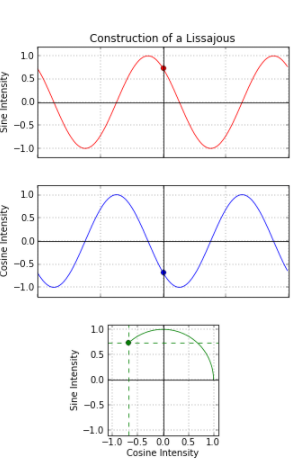
\includegraphics[width=\textwidth]{./img/Lissajous1.png}
  \end{minipage}
  \hfill
  \begin{minipage}[b]{0.49\textwidth}
    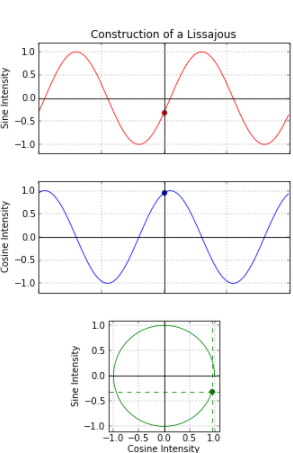
\includegraphics[width=\textwidth]{./img/Lissajous2.png}
  \end{minipage}
\end{figure}
\end{document}